%-------------------------------------------------------
%-                          包                           -%
%-------------------------------------------------------
\usepackage{ctex} % 自动处理中文和字体
\usepackage{url}
\usepackage[backend=biber,style=numeric-comp,sorting=none,gbpub=false,bibstyle=gb7714-2015,citestyle=gb7714-2015,
  gbpunctin=false,gbnamefmt=lowercase,
]{biblatex}

\usepackage{amsmath, amsfonts, amssymb}
\usepackage{booktabs} %三线表
\usepackage{threeparttable}
\usepackage{multicol}
\usepackage{multirow}
\usepackage{fancyhdr}
\usepackage{latexsym}
\usepackage{mathrsfs}
\usepackage{wasysym}
\usepackage{enumerate}
\usepackage{titlesec}
\usepackage{epstopdf}
\usepackage{caption}
\usepackage{graphicx, subfig} %图包
\usepackage{float}
\usepackage{setspace}
\usepackage{array}
\usepackage{fancyhdr} %页眉页脚包
\usepackage{titletoc} %设置目录格式
\usepackage{geometry} %设置页边距
% \usepackage{circledsteps}%enumerate带圈的序号
\usepackage{pifont}
\usepackage{adjustbox}

\usepackage[absolute,overlay]{textpos}
% \usepackage{tocloft}
\usepackage{hyperref} % href蓝链, 可以删除
\usepackage{pdfpages} % 插入pdf文件
\usepackage{makecell} % 

% 论文尺寸规格为A4(210×297mm)。每一面的上方(天头)和左侧(订口)应分别留边25mm,下方(地脚)和右侧(切口)应分别留边20mm。
\geometry{
  a4paper,
  left=25mm,
  right=20mm,
  top=25mm,
  bottom=20mm,
  % showframe,         % 保持开启以观察页面效果
  asymmetric         % 关键:强制所有页边距一致,不镜像
}
%论文尺寸为A4,全文页面设置为:上下2.54cm,左右3.17cm,含有大量图表可微调。页边距0.5cm
% \geometry{a4paper,left=3.17cm,right=3.17cm,top=2.54cm,bottom=2.54cm,bindingoffset=0.5cm} 

\setCJKmainfont{simsun.ttc} %文中中文为宋体
\setmainfont{Times New Roman} %文中英文为新罗马
\setlength{\baselineskip}{20pt} %行距为固定值20磅


%-------------------------------------------------------
%-                        字体设置                       -%
%-------------------------------------------------------
\setCJKfamilyfont{song}{simsun.ttc}
\setCJKfamilyfont{fs}{simfang.ttf}
\setCJKfamilyfont{kai}{simkai.ttf}
\setCJKfamilyfont{hei}{simhei.ttf}

\newcommand{\song}{\CJKfamily{song}}    % 宋体   (simsun.ttc)
\newcommand{\fs}{\CJKfamily{fs}}        % 仿宋体  (simfs.ttf)
\newcommand{\kai}{\CJKfamily{kai}}      % 楷体   (simkai.ttf)
\newcommand{\hei}{\CJKfamily{hei}}      % 黑体   (simhei.ttf)

%设置加粗体
%加粗楷体
\setCJKfamilyfont{kaitib}{simkai.ttf}[AutoFakeBold]
\newcommand{\kaitib}{\CJKfamily{kaitib}}
%加粗仿宋体
\setCJKfamilyfont{fangsongti}{simfang.ttf}[AutoFakeBold]
\newcommand{\fangsongti}{\CJKfamily{fangsongti}}
%加粗黑体
\setCJKfamilyfont{heitib}{simhei.ttf}[AutoFakeBold]
\newcommand{\heitib}{\CJKfamily{heitib}}
%加粗宋体
\setCJKfamilyfont{songtib}{simsun.ttc}[AutoFakeBold]
\newcommand{\songtib}{\CJKfamily{songtib}}
%正文加粗快捷键
\newcommand{\tbf}{\bfseries \songtib}
%-------------------------------------------------------
%-                          字号设置                     -%
%-------------------------------------------------------
\newcommand{\chuhao}{\fontsize{42pt}{\baselineskip}\selectfont}
\newcommand{\xiaochuhao}{\fontsize{36pt}{\baselineskip}\selectfont}
\newcommand{\yihao}{\fontsize{26pt}{\baselineskip}\selectfont}
\newcommand{\xiaoyihao}{\fontsize{24pt}{\baselineskip}\selectfont}
\newcommand{\erhao}{\fontsize{22pt}{\baselineskip}\selectfont}
\newcommand{\xiaoerhao}{\fontsize{18pt}{\baselineskip}\selectfont}
\newcommand{\sanhao}{\fontsize{16pt}{\baselineskip}\selectfont}
\newcommand{\xiaosanhao}{\fontsize{15pt}{\baselineskip}\selectfont}
\newcommand{\sihao}{\fontsize{14pt}{\baselineskip}\selectfont}
\newcommand{\xiaosihao}{\fontsize{12pt}{\baselineskip}\selectfont}
\newcommand{\wuhao}{\fontsize{10.5pt}{\baselineskip}\selectfont}
\newcommand{\xiaowuhao}{\fontsize{9pt}{\baselineskip}\selectfont}
\newcommand{\liuhao}{\fontsize{7.5pt}{\baselineskip}\selectfont}
\newcommand{\qihao}{\fontsize{5.5pt}{\baselineskip}\selectfont}
%-------------------------------------------------------
%-                       自定义枚举列表格式              -%
%-------------------------------------------------------
% 重定义第一级 enumerate 标签格式为 (1)
\renewcommand{\labelenumi}{(\theenumi)}
% 重定义第二级 enumerate 标签格式为 ①、②、③……
\renewcommand{\theenumii}{\arabic{enumii}} % 使用阿拉伯数字计数
\renewcommand{\labelenumii}{\textcircled{\theenumii}} % 将数字放入圈中
%-------------------------------------------------------
%-                        Chinesization                 -%
%-------------------------------------------------------
\newtheorem{theorem}{\hskip 2em定理}[section]
\newtheorem{definition}{\hskip 2em定义}[section]
\newtheorem{exam}{\hskip 2em例}[section]
\newtheorem{note}{\hskip 2em注}[section]
\newtheorem{proof}{{\it \hskip 2em\textbf{证明}}}[section]
\newtheorem{solution}{{\it \hskip 2em\textbf{解}}}
\renewcommand{\tablename}{\song 表}
\renewcommand{\figurename}{\song 图}
\renewcommand{\refname}{\centerline {参考文献}}
\renewcommand{\contentsname}{\fontsize{15.75pt}{\baselineskip}\selectfont \textbf{目~~~~录}}
\renewcommand{\thefootnote}{\arabic{footnote}}
\renewcommand{\theequation}{\thesection-\arabic{equation}}
\renewcommand{\thefigure}{\thesection-\arabic{figure}}
\renewcommand{\thetable}{\thesection-\arabic{table}}

%-------------------------------------------------------
%-                     公式随章编号                     -%
%-------------------------------------------------------
\date{}
\makeatletter
\renewcommand*\l@chapter[2]{%
  \ifnum \c@tocdepth >\m@ne
    \addpenalty{-\@highpenalty}%
    \vskip 1.0em \@plus\p@
    \setlength\@tempdima{1.5em}%
    \begingroup
    \parindent \z@ \rightskip \@pnumwidth
    \parfillskip -\@pnumwidth
    \leavevmode \bfseries
    \advance\leftskip\@tempdima
    \hskip -\leftskip
    #1\nobreak\leaders\hbox{$\m@th
        \mkern \@dotsep mu\hbox{-}\mkern \@dotsep
        mu$}\hfill \nobreak\hb@xt@\@pnumwidth{\hss #2}\par
    \penalty\@highpenalty
    \endgroup
  \fi}

% \date{}
% \numberwithin{equation}{section}
% \numberwithin{figure}{section}
% \numberwithin{table}{section}

%-------------------------------------------------------
%-                        Tabular Option                -%
%-------------------------------------------------------
\newcommand{\tabincell}[2]{\begin{tabular}{@{}#1@{}}#2\end{tabular}}
%-------------------------------------------------------
%-                        Caption Option                -%
%-------------------------------------------------------
\captionsetup[figure]{labelsep=space}
\captionsetup[table]{labelsep=space}
%-------------------------------------------------------
%-                        文献来源                       -%
%-------------------------------------------------------
\addbibresource{Text/reference.bib}
%-------------------------------------------------------
%-                        Page Control                  -%
%-------------------------------------------------------
% \topmargin=0cm \oddsidemargin=0.5cm \textwidth=15cm
% \textheight=22cm

%-------------------------------------------------------
%-                        目录格式配置                   -%
%-------------------------------------------------------
%目录正文:宋体5号,一级节标题加粗,行距17磅,段前0行,段后0行
%一级标题(如: 第一章 引言),首行不缩进
%二级标题(如:1.1研究背景及意义),首行缩进2个汉字
%三级标题(如:1.1.1研究背景),首行缩进4个汉字
\titlecontents{section}[0em]
{\fontsize{12pt}{\baselineskip}\selectfont}
{\hspace*{3em}\contentslabel{3em}\ }%
{}
{\titlerule*[0.7pc]{$\cdot$}\contentspage\hspace*{1em}}%

\titlecontents{subsection}[0em]
{\fontsize{12pt}{\baselineskip}\selectfont}
{\hspace*{3em}\contentslabel{1.5em}\ }% \hspace*{3em}效果不好
{}
{\titlerule*[0.7pc]{$\cdot$}\contentspage\hspace*{1em}}%

\titlecontents{subsubsection}[0em]
{\fontsize{12pt}{\baselineskip}\selectfont}
{\hspace*{4em}\contentslabel{2em}\ }%
{}
{\titlerule*[0.7pc]{$\cdot$}\contentspage\hspace*{1em}}%
\renewcommand{\baselinestretch}{1.1}


% 确保公式编号按章节划分,并包含章节号
% 例如,第一章的第一个公式是 (1-1) 或 (1.1) 取决于 \theequation 的定义
\numberwithin{equation}{section}

% 步骤 1: 将 \theequation 定义为纯数字编号部分 (例如: 1-1)
\renewcommand{\theequation}{\arabic{section}-\arabic{equation}}

% 步骤 2: 修改 \tagform@ 以自定义公式标签的显示格式
\makeatletter % 允许访问宏包内部命令
% #1 代表由 \theequation 生成的纯数字编号 (例如 "1-1")
% 我们将其格式化为 "公式 (#1)"
\def\tagform@#1{\maketag@@@{\text{公式 }(#1)\@@italiccorr}}
\makeatother


% -------------------------------------------------------
% -                       自定义命令                      -%
% -------------------------------------------------------
\makeatletter

\newcommand{\contenttitle}[1]{\def\@contenttitle{#1}}
\newcommand{\contenttitleSecond}[1]{\def\@contenttitleSecond{#1}}
\newcommand{\institute}[1]{\def\@institute{#1}}
\newcommand{\major}[1]{\def\@major{#1}}
\newcommand{\studentid}[1]{\def\@studentid{#1}}


\newcommand{\showtitle}{\@title}
\newcommand{\showcontenttitle}{\@contenttitle}
\newcommand{\showcontenttitleSecond}{\@contenttitleSecond}
\newcommand{\showinstitute}{\@institute}
\newcommand{\showmajor}{\@major}
\newcommand{\showstudentid}{\@studentid}




% 设置默认值,防止未定义时报错
\providecommand{\@contenttitle}{记得填写标题!}
\providecommand{\@contenttitleSecond}{\@empty}
\providecommand{\@institute}{记得填写学院!}
\providecommand{\@major}{记得填写专业!}
\providecommand{\@studentid}{记得填写学号!}



\newcolumntype{M}[1]{>{\centering\arraybackslash}m{#1}} % 水平居中的m列
\newcolumntype{B}[1]{>{\centering\arraybackslash}b{#1}} % 水平居中的b列

\makeatother

% -------------------------------------------------------
% -                       自定义封面命令                  -%
% -------------------------------------------------------
\makeatletter
\renewcommand{\maketitle}{
    \pagestyle{empty}\fancyhf{}
    \begin{titlepage}
        % 复制word的图片, 尽管测量了距离, 还是有一点误差
        % \begin{textblock*}{\textwidth}(\dimexpr (\paperwidth - \textwidth) / 2 \relax, 3.85cm) %距离页面顶部距离3.85cm
        %     \begin{figure}[H]
        %         \centering
        %         
\includegraphics[height=2.25cm, keepaspectratio]{TemplateAssets/fzu1.png}
        %         \hspace{0.55cm}
        %         
\includegraphics[height=2.25cm, keepaspectratio]{TemplateAssets/fzu2.png}
        %         \hspace{0.55cm}
        %         
\includegraphics[height=2.25cm, keepaspectratio]{TemplateAssets/fzu3.png}
        %         \hspace{0.74cm}
        %         
\includegraphics[height=2.25cm, keepaspectratio]{TemplateAssets/fzu4.png}
        %     \end{figure}
        % \end{textblock*}

        % 矢量图版本, 使用校徽的矢量图, 对每个字添加了等高且等距的轮廓后, 放大到word封面相同高度
        % 但是发现学校下发的word封面可能并没有严格等距...
        \begin{textblock*}{\textwidth}(\dimexpr (\paperwidth - \textwidth) / 2 \relax, 4.10cm) %距离页面顶部距离4.10cm
            \begin{figure}[H]
                \centering
                
\includegraphics[height=1.85cm, keepaspectratio]{TemplateAssets/fzu1.pdf}
                \hspace{0.56cm}
                
\includegraphics[height=1.85cm, keepaspectratio]{TemplateAssets/fzu2.pdf}
                \hspace{0.56cm}
                
\includegraphics[height=1.85cm, keepaspectratio]{TemplateAssets/fzu3.pdf}
                \hspace{0.56cm}
                
\includegraphics[height=1.85cm, keepaspectratio]{TemplateAssets/fzu4.pdf}
            \end{figure}
        \end{textblock*}

        % \newcolumntype{M}[1]{>{\centering\arraybackslash}m{#1}}
        % \newcolumntype{B}[1]{>{\centering\arraybackslash}b{#1}}

        \begin{textblock*}{\textwidth}(\dimexpr (\paperwidth - \textwidth) / 2 \relax, 8.08cm)
            \begin{center}
                %中文题目:宋体1号字
                % \linespread{1.5}\selectfont %设置行距
                \tbf \yihao \hspace{1.2cm}\@title
            \end{center}
        \end{textblock*}

        \begin{textblock*}{\textwidth}(\dimexpr (\paperwidth - \textwidth) / 2 \relax, 10.6cm)
            {
                    %学科专业等:宋体3号字
                    \song \sanhao
                    \setlength{\tabcolsep}{0.12cm}
                    \begin{center}
                        \begin{tabular}[b]{B{3cm} B{9.18cm}}
                            {题\hspace{1.1cm}目:} & {\@contenttitle}       \\\Xcline{2-2}{1pt}       \\[0.24cm]
                            {}                  & {\@contenttitleSecond} \\  \Xcline{2-2}{1pt}                   \\[0.24cm]
                            {姓\hspace{1.1cm}名:} & {\@author}             \\\Xcline{2-2}{1pt}    \\[0.45cm]
                            {学\hspace{1.1cm}号:} & {\@studentid}          \\\Xcline{2-2}{1pt}    \\[0.45cm]
                            {学\hspace{1.1cm}院:} & {\@institute}          \\\Xcline{2-2}{1pt}    \\[0.45cm]
                            {专\hspace{1.1cm}业:} & {\@major}              \\\Xcline{2-2}{1pt}    \\[0.45cm]
                            {年\hspace{1.1cm}级:} & {2021级}                \\\Xcline{2-2}{1pt}    \\[0.45cm]
                        \end{tabular}

                        \vspace{-0.17cm}

                        \begin{tabular}[b]{B{4.1cm} B{6.03cm} B{2cm}}
                            {校内指导教师:} &
                            % 在这里插入校内导师签名图片
                            % 替换为你的签名图片, e.g., Fig/signature_internal.png
                            \raisebox{-0.3\height}{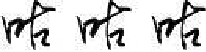
\includegraphics[height=0.8cm, keepaspectratio]{TemplateAssets/example-signature.pdf}}
                                      & {(签名)} \\\Xcline{2-2}{1pt}\\[0.45cm]  % 空白行
                            {校外指导教师:} &
                            % 在这里插入校外导师签名图片, 如没有, 可以注释该行
                            % 替换为你的签名图片, e.g., Fig/signature_external.png
                            % \raisebox{-0.3\height}{\includegraphics[height=0.8cm, keepaspectratio]{example-image}} 
                                      & {(签名)} \\\Xcline{2-2}{1pt} \\[0.45cm]  % 空白行
                        \end{tabular}
                    \end{center}

                    \begin{center}
                        \song \sanhao
                        \hspace{8em}\@date
                    \end{center}
                }
        \end{textblock*}
        \ %
    \end{titlepage}
    \newpage
}
\makeatother % 自定义封面命令